\chapter{Titans}
\label{chap:titans}

Titans are mech-style robots, descended from modern-day fledgling military exoskeletons, designed for both civilian and military applications. 

There are three classes of titans, as described below.

\section{Special Rules}
\label{sec:specialrules}

All titans have the following special rule:

\textbf{Mecha Chassis:} As long as a Titan's propulsion isn't compromised it ignores the speed requirement for the reposition maneuver.

\section{Stryder}
\label{sec:stryder}
\begin{wrapfigure}[13]{r}{.34\linewidth}
\vspace*{-2em}
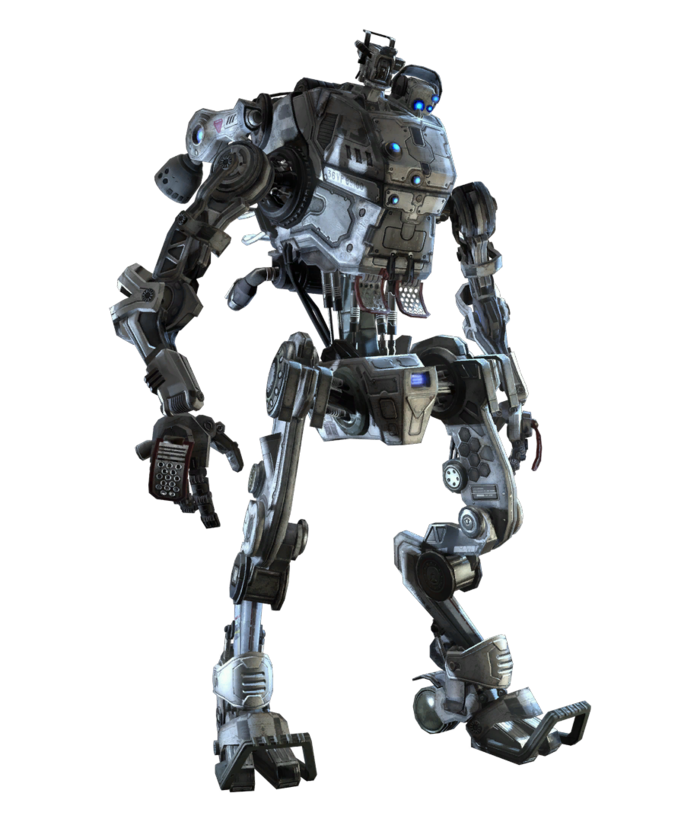
\includegraphics[width=\linewidth]{Stryder}
\end{wrapfigure}


The Stryder is a Titan chassis developed and manufactured by Hammond Robotics. Developed as an extremely mobile and maneuverable Titan variant, the Stryder's almost skeletal design has been optimized for superior speed and agility. Significant improvements have been made to its Dash Core, while the Titan can also sprint for greater distances, making it perfect for hit-and-run attacks, ambushes and rapid redeployments. Unfortunately, this speed comes at a price. The Stryder's design is stripped down compared to other Titan variants, and its armor is largely non-existent, making it much more fragile in combat. In Titan-vs-Titan engagements, Stryder Pilots must use all available cover and their machine's impressive speed to outflank and evade their heavier adversaries, as they are unlikely to survive a straight-up slug-fest.

\textbf{Dash Core}: The Stryder-class Titan has an in-built dash core. Once per round on your turn, you may cause the titan to suffer 1 system strain to perform the Evade maneuver as an Incidental, ignoring the Speed requirement.

\vspace{2em}

\Vehicle{3}{3}{+2}{2}{1}{13}{20}

\begin{multicols}{2}
\noindent\textbf{Control Skill:} Pilot (Titan)\\
\noindent\textbf{Complement:} One pilot\\
\noindent\textbf{Passenger Capacity:} None\\
\noindent\textbf{Price/Rarity:} 20,750/8\\
\noindent\textbf{Consumables:} None\\
\noindent\textbf{Encumbrance Capacity:} 2\\
\noindent\textbf{Weapons:} Titan punch (Pilot [Titan]; Damage 2; Critical 3; Range [Engaged]; Accurate 1)\\
\noindent\textbf{Hard Points:} 3
\end{multicols}

\section{Atlas}
\label{sec:atlas}
\begin{wrapfigure}{l}{.34\linewidth}
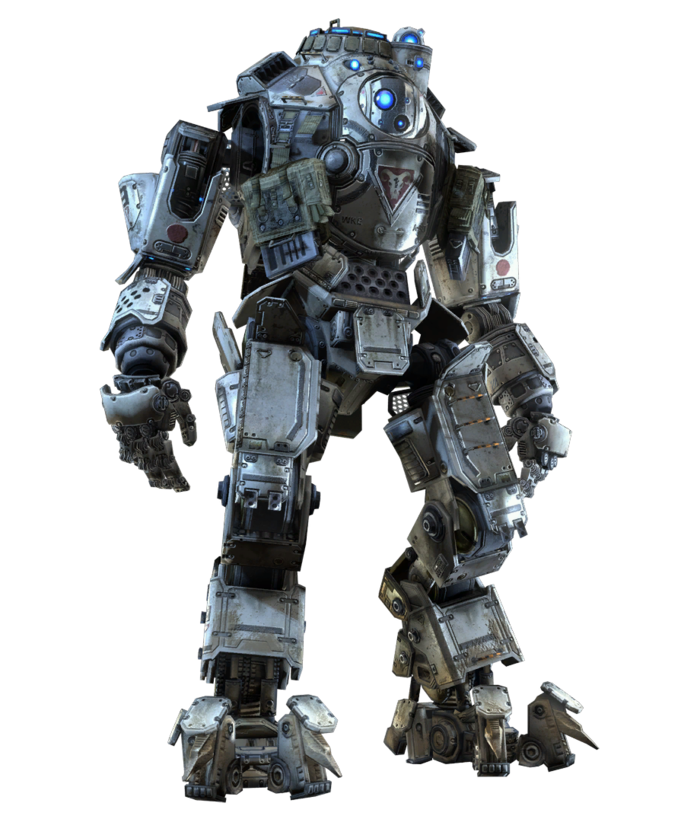
\includegraphics[width=\linewidth]{Atlas}
\end{wrapfigure}


The Atlas is the original Titan model produced by Hammond Robotics. It has a balance of mobility and armor, having more mobility than the Ogre, but more armor than the Stryder. This was the first Titan to be revealed.

The Atlas seems to be the second tallest Titan model, though exact measurements are unknown. Based on photos of the Atlas standing next to a pilot, it can be estimated to be between 20-25 feet tall. Its main entry point is in its chest, which opens up for the player. The Atlas also has a secondary entry point---a small hatch in the top. This is also the eject port for the Atlas.

The Atlas is the oldest Titan model on the Frontier and has instigated the development of both the Stryder and Ogre patterns. It was used through the Titan Wars, and onto the Frontier War. The Atlas is equipped with a Damage Core, which, when ready, the pilot can activate on command to substantially increase damage dealt by the titan.

\textbf{Damage Core}: The Atlas-class Titan has an in-built damage core. Once per round on your turn, you may cause the titan to suffer 1 system strain to perform the Aim maneuver as an Incidental.\\[1em]

\Vehicle{3}{2}{+0}{2}{2}{15}{15}

\begin{multicols}{2}
\noindent\textbf{Control Skill:} Pilot (Titan)\\
\noindent\textbf{Complement:} One pilot\\
\noindent\textbf{Passenger Capacity:} None\\
\noindent\textbf{Price/Rarity:} 21,750/8\\
\noindent\textbf{Consumables:} None\\
\noindent\textbf{Encumbrance Capacity:} 2\\
\noindent\textbf{Weapons:} Titan punch (Pilot [Titan]; Damage 2; Critical 3; Range [Engaged])\\
\noindent\textbf{Hard Points:} 3
\end{multicols}

\vspace*{\fill}
\pagebreak

\section{Ogre}
\label{sec:ogre}
\begin{wrapfigure}[12]{r}{.34\linewidth}
\vspace*{-2em}
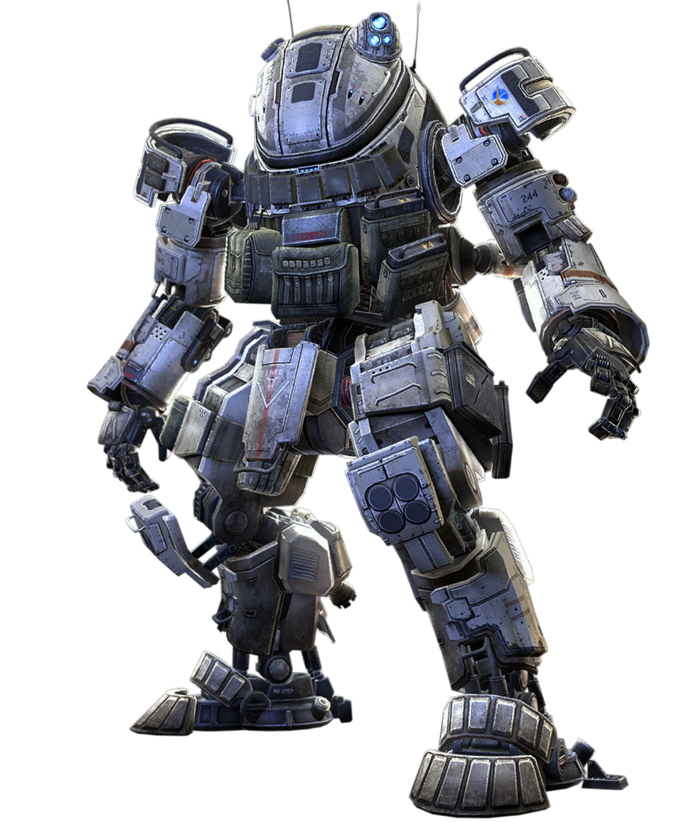
\includegraphics[width=\linewidth]{Ogre}
\end{wrapfigure}

The H-KA02/a Ogre Heavy Titan is a Titan model produced by Hammond Armament Division and Wonyeon Defense. Developed as an extremely tough Titan chassis, the Ogre's design has been compared to a main battle tank, optimized for taking higher amounts of damage and dealing out more than the Atlas or Stryder Titans. The Ogre stands slightly taller than the Atlas and has bulkier armor. The main entry point of an Ogre is via a large hatch on its top rather than the chest, like the Atlas or Stryder. The Ogre is equipped with a Shield Core, which amps the Titan's shield for a limited time.

\textbf{Shield Core}: The Ogre-class Titan has an in-built shield core. Once per round on your turn, you may cause the titan to suffer 1 system strain to perform the Brace for Impact maneuver as an Incidental.\\[3em]

\Vehicle{3}{1}{-2}{2}{2}{18}{18}


\begin{multicols}{2}
\noindent\textbf{Control Skill:} Pilot (Titan)\\
\noindent\textbf{Complement:} One pilot\\
\noindent\textbf{Passenger Capacity:} None\\
\noindent\textbf{Price/Rarity:} 25,740/8\\
\noindent\textbf{Consumables:} None\\
\noindent\textbf{Encumbrance Capacity:} 2\\
\noindent\textbf{Weapons:} Titan punch (Pilot [Titan]; Damage 2; Critical 3; Range [Engaged]; Vicious 1)\\
\noindent\textbf{Hard Points:} 3
\end{multicols}



No Titan is complete without its weapons. Most Titans have one primary, handheld weapon, one ordnance launcher and one defensive system. Some pilots prefer to change it up a bit and go for extra defense or offense. 

\section{Titan Weapons}

Each main weapon takes up one hard point on the Titan. Titan primary weapons follow the same rules as personal-scale weapons with regards to ammo. Unless you get an out of ammo result due to a \Despair\ (or \Threat\Threat\Threat\ for some weapons) the Titan is assumed to carry enough reloads to not worry about them.

Titan ordnance, on the other hand, has a limit to how much can be stored in a launcher at a time. Once all ammo is fired, that's it until the Titan can be rearmed at an appropriate facility. Note that you can install the Extra Ammo attachment to provide one reload for one installed ordnance weapon.

\subsection{40mm Cannon}

\begin{wrapfigure}[3]{l}{.34\linewidth}
\vspace*{-2em}
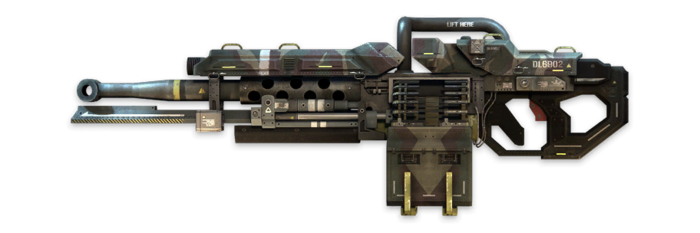
\includegraphics[width=\linewidth]{40mmCannon}
\end{wrapfigure}

The factory issue 40mm Cannon is a semi-automatic weapon that fires a high-explosive round with good accuracy. 

\subsection{Arc Cannon}
\begin{wrapfigure}[4]{r}{.34\linewidth}
\vspace*{-2em}
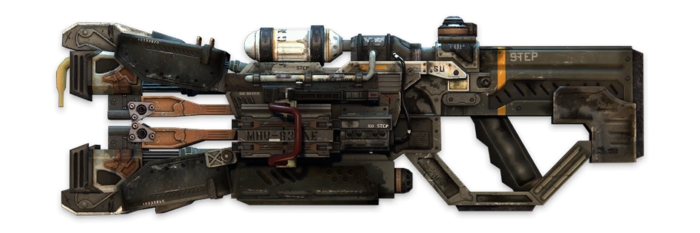
\includegraphics[width=\linewidth]{ArcCannon}
\end{wrapfigure}

The factory issue Arc Cannon fires a bolt of lightning that propagates across multiple targets. It can be fired quickly, or charged up over time for an increase in firepower. If you perform the Prepare maneuver, increase the damage of one hit of the next combat check by 1 and an arc cannon can negate Defense granted by energy shields by spending \Advantage\Advantage.

\subsection{PR-01 Plasma Railgun}
\begin{wrapfigure}[3]{l}{.34\linewidth}
\vspace*{-2em}
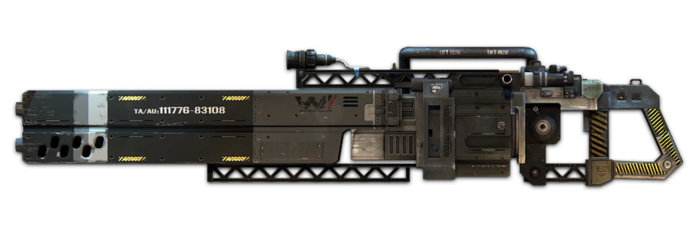
\includegraphics[width=\linewidth]{PlasmaRailgun}
\end{wrapfigure}

The Plasma Railgun is a Titan-sized sniper weapon, used for suppression of armored targets from a distance. The weapon fires a bolt of plasma, accelerated by a system of charged rails.


\subsection{Quad Rocket}
\begin{wrapfigure}[2]{r}{.34\linewidth}
\vspace*{-2em}
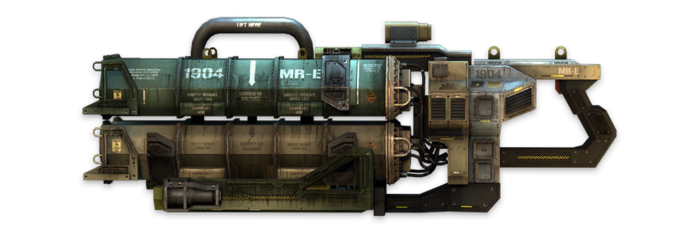
\includegraphics[width=\linewidth]{QuadRocket}
\end{wrapfigure}

The Quad Rocket is a weapon that fires a tight-knit cluster of 4 rockets at the target, exploding upon impact.

\subsection{Triple Threat}
\begin{wrapfigure}[4]{l}{.34\linewidth}
\vspace*{-2em}
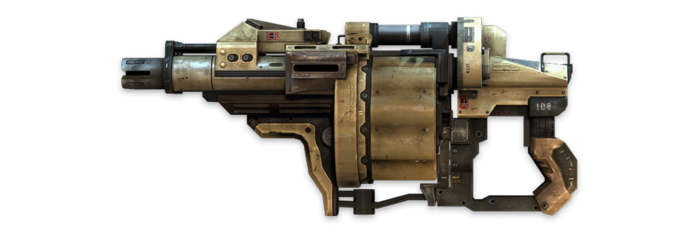
\includegraphics[width=\linewidth]{TripleThreat}
\end{wrapfigure}

The Triple Threat is a grenade launcher that shoots 3 grenades at once. It excels at clearing rooms, and its grenades explode on armored contact, making it effective at close range against other Titans. Due to the low magazine capacity, however, this weapon can run out of ammo by spending \Threat\Threat\Threat\ (instead of the normal \Despair).

\subsection{XOTBR-16 Chaingun}
\begin{wrapfigure}[3]{r}{.34\linewidth}
\vspace*{-2em}
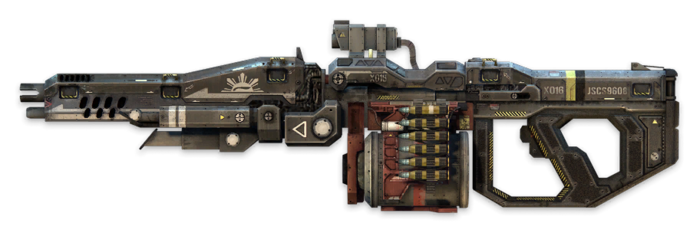
\includegraphics[width=\linewidth]{XO16Chaingun}
\end{wrapfigure}

The XO-16 Chaingun is a fully automatic ballistic weapon that fires 1.6 inch slugs with high precision at considerable range.

\begin{table}[h!]
\caption{Titan Weapons}
\footnotesize
\begin{GenesysTable}{*{2}{l} *{2}{c} l c r c X[l]}
Name & Skill & Dam & Crit & Range  & HP & Price & Rarity & Special\\
40mm Cannon & Gunnery & 6 & 3 & Long & 1 & 7,750 & 6 & Blast 1, Breach 1 \\
Arc Cannon & Gunnery & 4 & 4 & Medium & 1 & 5,250 & 7 & Blast 3, Special\\
Plasma Railgun & Gunnery & 7 & 2 & Extreme & 1 & 10,750 & 7 & \Special{Accurate 1, Breach 1, Limited Ammo 2}
Quad Rocket & Gunnery & 4 & 3 & Long & 1 & 7,500 & 6 & \Special{Accurate 1, Blast 3, Vicious 2}
Triple Threat & Gunnery & 4 & 4 & Medium & 1 & 8,250 & 7 & \Special{Blast 2, Linked 2, Special}
XO-16 Chaingun & Gunnery & 3 & 4 & Long & 1 & 4,750 & 7 & Auto-fire
\end{GenesysTable}
\end{table}

\section{Titan Ordnance}
Unless otherwise noted, extra reloads for ordnance weapons cost 2,000 credits.

\subsection{Cluster Missile}
\begin{wrapfigure}[4]{l}{.34\linewidth}
\vspace*{-2em}
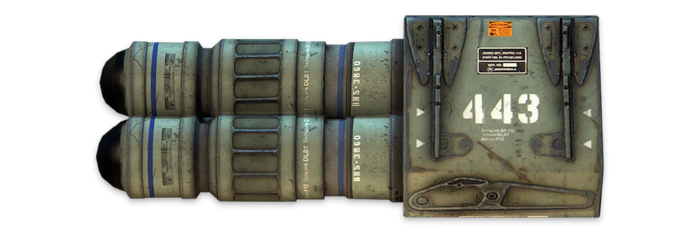
\includegraphics[width=\linewidth]{ClusterMissile}
\end{wrapfigure}

The Cluster Missile pod fires a missile which, on impact, deploys a shower of secondary explosive charges that continue to explode and saturate an area for a considerable time.

\subsection{Laser Shot}
The laser shot fires a lethal beam that cuts through anything in its way. It's a directed energy weapon that takes the charge rifle and and amps it up to Titan-scale.

\subsection{Multi-Target Missile System}
\begin{wrapfigure}[3]{r}{.34\linewidth}
\vspace*{-2em}
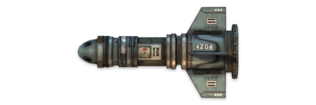
\includegraphics[width=\linewidth]{MultiTargetMissileSystem}
\end{wrapfigure}

The Multi-Target Missile System enables you to engage multiple targets at once. The Guided quality can only be activated when attacking targets made of significant metal content, like Titans and Spectres.

\subsection{Rocket Salvo}
\begin{wrapfigure}[2]{l}{.34\linewidth}
\vspace*{-2em}
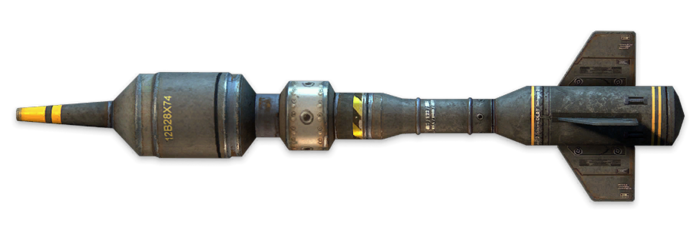
\includegraphics[width=\linewidth]{RocketSalvo}
\end{wrapfigure}

The Rocket Salvo launches a rapid salvo of unguided rockets. Each \Success\  deals +2 damage, instead of +1.

\subsection{Slaved Warheads}
\begin{wrapfigure}[3]{r}{.34\linewidth}
\vspace*{-2em}
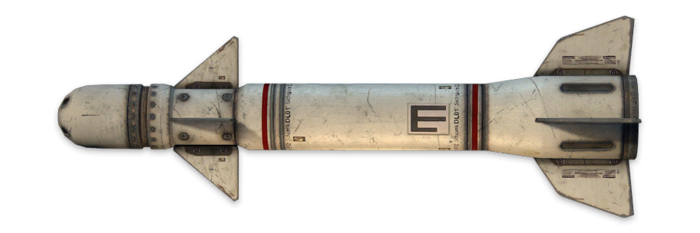
\includegraphics[width=\linewidth]{SlavedWarheads}
\end{wrapfigure}

This Titan ordnance pod requires a lock-on before you can fire. When you fire, a barrage of 3 homing missiles will launch towards your locked target. The Guided quality can only be activated when attacking targets made of significant metal content, like Titans and Spectres.


\begin{table}[h!]
\caption{Titan Ordnance}
\footnotesize
\begin{GenesysTable}{*{2}{l} *{2}{c} l c r c X[l]}
Name & Skill & Dam & Crit & Range  & HP & Price & Rarity & Special\\
Cluster Missile & Gunnery & 4 & 3 & Extreme & 1 & 6,250 & 8 & \Special{Blast 4, Breach 1, Limited Ammo 3}
Laser Shot & Gunnery & 3 & 2 & Long & 1 & 5,100 & 8 & \Special{Accurate 1, Breach 2, Slow-Firing 1, Vicious 2}
MTM System & Gunnery & 5 & 3 & Extreme & 1 & 9,000 & 8 & \Special{Accurate 1, Auto-Fire, Breach 1, Guided 3, Limited Ammo 3, Special}
Rocket Salvo & Gunnery & 3 & 2 & Long & 1 & 7,050 & 8 & \Special{Blast 1, Breach 2, Inaccurate 1, Limited Ammo 2, Special}
Slave Warhead & Gunnery & 5 & 4 & Long & 1 & 8,250 & 8 & \Special{Blast 1, Breach 1, Guided 2, Limited Ammo 3, Linked 2}
\end{GenesysTable}
\end{table}


\section{Defensive Systems}
Titans are not indestructible, regardless of what the IMC wants you to believe. Each Titan is equipped with one of three defensive systems, designed to prolong the lifespan of the Titan.


\subsection{Electric Smoke}
\begin{wrapfigure}[6]{l}{.25\linewidth}
\vspace*{-2em}

\includegraphics[width=\linewidth]{ElectricSmoke}
\end{wrapfigure}

Electric smoke is a reactionary device used to avoid attacks and negate tracking weapons.

Once per round, as an out-of-turn incidental, you may deploy a smoke charge. If this was done as a reaction to being targeted by a Guided weapon, the tracking is lost and the weapon may not fire on your Titan this turn. It creates an area of obscurant around your Titan that grants concealment worth +3 dice (see page 110 of the \emph{Genesys} Core Rulebook).Any pilot on your Titan must immediately move away from your Titan or risk taking damage from the electric smoke. If they won't (or can't) disembark, they must make a \textbf{Hard (\DifficultyDie\DifficultyDie\DifficultyDie) Resilience check} or suffer 1 wound, plus 1 additional wound per \Failure. If the Resilience check generates \Threat\Threat, they become Disoriented for two rounds. This cloud lasts until the end of your next turn. Any pilot that ends their turn in the smoke must make the Resilience check or suffer wound as described above.

If the skill check that triggered the electric smoke generates \Advantage\Advantage, it may be spent to cause you to have only one smoke canister left.

\subsection{Partical Wall}
\begin{wrapfigure}[6]{r}{.25\linewidth}
\vspace*{-4em}

\includegraphics[width=\linewidth]{ParticleWall}
\end{wrapfigure}

The particle wall creates a concave force field which blocks all projectiles from one side and lets all projectiles through from the other. As an incidental you may deploy the particle wall in front of your Titan. It grants Ranged Defense 4 to all Titans behind the wall. It lasts until the end of your next turn, and it requires two rounds to recharge before it can be used again.

\subsection{Vortex Shield}
\begin{wrapfigure}[7]{l}{.25\linewidth}
\vspace*{-2em}

\includegraphics[width=\linewidth]{VortexShield}
\end{wrapfigure}

The Vortex Shield allows Titans to stop enemy fire such as rockets and bullets in their tracks and is able to send the projectiles right back to the enemy.

As an out-of-turn incidental you may deploy the vortex shield when targeted by a ranged combat check. It provides the Reflective 1 quality until the beginning of your next turn. If the triggering attack generates \Threat\Threat\Threat, you may reflect the projectile (if any) back on the target, dealing the weapon's base damage to the attacker. If the check generates \Despair, you instead deal a Critical Injury (or a Critical Hit for vehicles).

\begin{table}[h!]
\centering
\caption{Titan Defensive Systems}
\footnotesize
\begin{GenesysTable}{*{2}{l} *{2}{c} l c r c X[l]}
System & Hard Point & Price & Rarity\\
Electric Smoke & 1 & 2,000 & 8\\
Particle Wall & 1 & 3,000 & 8\\
Vortex Shield & 1 & 1,000 & 8
\end{GenesysTable}
\end{table}